% Preamble
\documentclass[xcolor=dvipsnames]{beamer}
\usetheme{madrid}

% Packages
\usepackage[english,ngerman]{babel}
\usepackage[utf8]{inputenc}
\usepackage{amsmath}
\usepackage{graphicx}
\usepackage{hyperref}

\definecolor{hBlue}{RGB}{55,118,165}
\usecolortheme[named=hBlue]{structure}

\titlegraphic{
\includegraphics[width=4cm]{../images/logo.png}}
\title{Gesundheit \& Ernährung}
\subtitle{21-Tage-Kur}
\author{Adrian Helberg}
\date{03.05.2021}

% Document
\begin{document}

    \maketitle

    \frame{\frametitle{Agenda}\tableofcontents}

    \section{Einleitung}
    {
        \setbeamercolor{normal text}{fg=hBlue}\usebeamercolor*{normal text}
        \begin{frame}
            \begin{center}
                \Huge Einleitung
            \end{center}
        \end{frame}
    }

    \subsection{Langfristiges Ziel}
    \begin{frame}[allowframebreaks]
        \frametitle{Langfristiges Ziel}
        \begin{block}{Teufelskreis durchbrechen}
            \begin{itemize}
                \setlength\itemsep{1em}
                \item unreflektierte Kohlenhydratisierung verhindern\\ "`Blutzucker hochjagen"'
                \item Weg ebnen für eine natürliche Funktion des Körpers
                \item Hormone ins Gleichgewicht bringen
                \item Organsystem entlasten
            \end{itemize}
        \end{block}

        \framebreak

        \begin{block}{Was können wir erwarten?}
            \begin{itemize}
                \setlength\itemsep{1em}
                \item Sättigende Ernährung
                \item Gesundheit bis ins hohe Alter
                \item Lebensqualität
                \item Keine chronischen Krankheiten (Zivilisationskrankheiten)
                \item Natürliches Schlanksein
            \end{itemize}
        \end{block}
    \end{frame}

    \subsection{Kurzfristiges Ziel}
    \begin{frame}
        \frametitle{Kurzfristiges Ziel - 21-Tage-Kur}

        \begin{block}{Hormone - Hauptdarsteller}
            \begin{itemize}
                \setlength\itemsep{1em}
                \item Insulin
                \item Leptin
                \item Glukagon
                \item Cortisol
            \end{itemize}
        \end{block}
    \end{frame}

    \section{Vorbereitung}
    {
    \setbeamercolor{normal text}{fg=hBlue}\usebeamercolor*{normal text}
    \begin{frame}
        \begin{center}
            \Huge Vorbereitung
        \end{center}
    \end{frame}
    }

    \subsection{Mentale Vorbereitung}
    \begin{frame}[allowframebreaks]
        \frametitle{Mentale Vorbereitung}

        \begin{block}{"`Menschen sind Gewohnheitstiere"'}
            \begin{itemize}
                \setlength\itemsep{1em}
                \item Vehemente Verteidigung der Gewohnheiten (des Körpers)
                \item kein Gesunheitsfreak, sondern ein gesunder Mensch mit Lebensqualität
                \item Urlaub / Wochenende als "`Stunde Null"'
            \end{itemize}
        \end{block}

        \framebreak

        \begin{block}{Motive finden -  Was will ich erreichen?}
            \begin{itemize}
                \setlength\itemsep{1em}
                \item Abnehmen
                \item Spaß an Bewegung haben
                \item Leistungsfähiger sein
                \item Selbstbewusstsein stärken
                \item Messwerte (z.B. Blutdruck) verbessern
                \item Attraktivität steigern
                \item Schmerzen lindern
                \item Mit anderen "`mithalten"' können
            \end{itemize}
        \end{block}

    \end{frame}

    \subsection{Körperliche Vorbereitung}
    \begin{frame}[allowframebreaks]
        \frametitle{Körperliche Vorbereitung}

        \begin{block}{Bestandsaufnahme}
            \begin{itemize}
                \setlength\itemsep{1em}
                \item Werte messen: Gewicht, Bauchumfang (Körperfettanteil, Laborwerte?)
                \item Mahlzeiten planen, Einkaufen
                \item Guter Schlaf (Social-Jetlag-Syndrome)
                \item Kühlschrank ausmisten
                \item Protokoll führen?
            \end{itemize}
        \end{block}

        \framebreak

        \underline{Auf was muss ich achten? Was fliegt raus?}
        \begin{itemize}
            \setlength\itemsep{1em}
            \item Flüssige Nahrung
            \item Light-Produkte
            \item Süßigkeiten
            \item Fertiggerichte
            \item komplexe Kohlenhydrate (Kartoffeln, Nudeln, Brot)
            \item Produkte mit Zuckerzusatz
            \item Emulgatoren, "`E-Nummern"'
        \end{itemize}
    \end{frame}


    \section{Phase 1 (21 Tage)}
    {
        \setbeamercolor{normal text}{fg=hBlue}\usebeamercolor*{normal text}
        \begin{frame}
            \begin{center}
                \Huge Phase 1 (21 Tage)
            \end{center}
        \end{frame}
    }

    \subsection{Ziel}
    \begin{frame}
        \frametitle{Ziel}
        "`Zucker raus, Heißhunger abstellen, Darm schützen"'
        \begin{block}{Warum ist diese Phase entscheidend?}
            \begin{itemize}
                \setlength\itemsep{1em}
                \item Reset-Knopf drücken
                \item Probleme "`bei der Wurzel packen"'
                \item Entzündungen abbauen
            \end{itemize}
        \end{block}
    \end{frame}

    \subsection{Regeln}
    \begin{frame}
        \frametitle{Regeln}
        \begin{itemize}
            \setlength\itemsep{1em}
            \item Richtiges Essen: Satt werden, Kauen, Essen \& Trinken trennen
            \item 2-3 Feste Mahlzeiten (kein Snacken) nach "`Tellerprinzip"'
            \item Nahrungsmitteln nach GLYX-Tabelle
            \item Weiterhin "`das perfekte Frühstück"'
            \item Reichlich Wasser trinken
            \item Kein Alkohol
            \item Nach dem Aufwachen mind. 2 Gläser Wasser
            \item Vitamin D3 !
        \end{itemize}
    \end{frame}

    \subsection{GLYX}
    \begin{frame}
        \frametitle{GLYX - Glykämische Last}
        \begin{figure}
            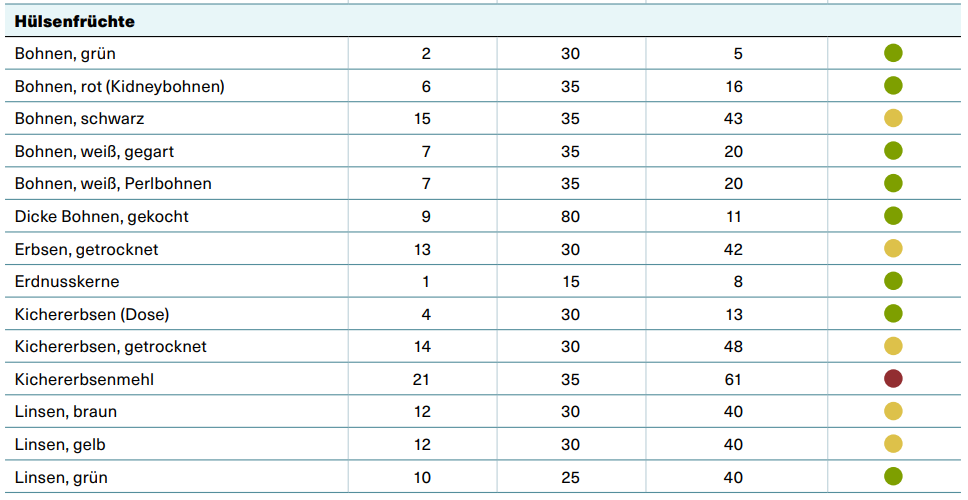
\includegraphics[width=10cm]{../images/glyx.png}
            \caption{GLYX-Tabelle nach Dr. Anne Fleck \url{https://bjvv.de/Files/PDF/GLYX-Liste_Schlank_Auflage4_gesch.pdf}}
        \end{figure}
    \end{frame}

    \section{Phase 2}
    {
        \setbeamercolor{normal text}{fg=hBlue}\usebeamercolor*{normal text}
        \begin{frame}
            \begin{center}
                \Huge Phase 2
            \end{center}
        \end{frame}
    }

    \subsection{Ziel}
    \begin{frame}
        \frametitle{Ziel}
        \begin{block}{Einführung von Kohlenhydraten}
            \begin{itemize}
                \setlength\itemsep{1em}
                \item Gute, langkettige Kohlenhydrate können wieder aufgenommen werden
                \item Kohlenhydrate nach Grad der körperlichen Betätigung
            \end{itemize}
        \end{block}

    \end{frame}

\end{document}
